\documentclass{article}

\usepackage[T1]{fontenc}
\usepackage{iclr2026_conference,times}
\usepackage{amsmath,amssymb,booktabs,float,graphicx,microtype,array}
% R173: \seqsplit was removed. It inserted break opportunities inside words, so the
% extracted PDF text layer contained mid-word splits ("PARTIALL Y", broken script
% names) and long paths were unsearchable. Code spans now break only at path
% separators, marked explicitly with \zb, so every word survives extraction intact.
\newcommand{\zb}{\discretionary{}{}{}}
\newcommand{\code}[1]{\texttt{#1}}

\usepackage[hidelinks]{hyperref}
\renewcommand{\topfraction}{0.92}
\renewcommand{\textfraction}{0.06}
\renewcommand{\floatpagefraction}{0.80}
% R236: 5pt rather than 7pt. Seven floats carry three separations each in the worst case, and
% this is float whitespace only -- no float, caption, row or value is touched.
\setlength{\textfloatsep}{5pt plus 2pt minus 2pt}
\setlength{\floatsep}{5pt plus 2pt minus 2pt}
\setlength{\intextsep}{5pt plus 2pt minus 2pt}
\setlength{\abovedisplayskip}{5pt plus 2pt minus 2pt}
\setlength{\belowdisplayskip}{5pt plus 2pt minus 2pt}
\setlength{\abovedisplayshortskip}{3pt plus 2pt}
\setlength{\belowdisplayshortskip}{3pt plus 2pt}
% Table captions sit above the tabular, and article's default \belowcaptionskip=0pt
% lets \toprule touch the caption's last line, which reads as an underline. Move 4pt
% from above to below so the separation appears at no net float height.
\setlength{\abovecaptionskip}{4pt plus 1pt minus 1pt}
\setlength{\belowcaptionskip}{4pt}

% R236 page-fit, layout only. The R174 audit fix that prints both data figures 1:1 at
% \textwidth (so their 7pt artwork labels stay 7pt) costs vertical space, which pushed the
% closing lines of the Conclusion onto a tenth main-text page. The space is recovered from
% inter-block whitespace, not from content: article's default list pays \topsep+\partopsep
% (~10pt) above and \topsep below every displayed list, and four such lists carry the main
% text. Patched through \list so it also applies inside the \footnotesize block; every
% bullet, value, scope label and claim is unchanged.
\makeatletter
\let\p@outerlist\list
\def\list#1#2{\p@outerlist{#1}{#2\setlength{\topsep}{2\p@ plus1\p@ minus1\p@}%
  \setlength{\partopsep}{\z@}}}
% The captions carry the scope discipline, so none of them is shortened; they are set
% one size step down instead (9pt on 11pt). That is still larger than the 8pt artwork labels
% the R270 audit fix installed, and it recovers the remaining lines the 1:1 figures cost.
\let\p@origmakecaption\@makecaption
\long\def\@makecaption#1#2{\begingroup\small\p@origmakecaption{#1}{#2}\endgroup}
\makeatother

\pagestyle{fancy}

% Break the title where its clauses break. Letting the first line fill \textwidth
% justified it, which printed visibly uneven small-caps word spacing (R174 audit).
\title{A NOT\_MEASURED Register\\for a Withdrawn KV-Selective Serving Study:\\Scope, Frozen Values, and a Guarded Rerun}

\author{Anonymous Author(s)\\
Affiliation withheld for double-blind review\\
}
\date{}

\begin{document}
\raggedbottom

\maketitle

\begin{abstract}
We document the withdrawal of a frozen repeated-query serving study whose evidence did not
support its original cost--quality interpretation.  The note contributes three reporting
instruments: scoped statements for each surviving claim, a \textbf{NOT\_MEASURED register}
that is complete relative to an author-enumerated claim ledger (not an independent ground
truth; Section~\ref{sec:reg}), and frozen values with per-row scope labels.  Pattern-enumerated
checks make violations within their declared phrasing universe re-runnable, while leaving
coverage outside that universe explicitly open.

Static audit identified two application-level defects that had previously been read as
hardware boundaries: a thread-local grad-mode leak in the full-context worker
($\approx$2 lines, fixed and re-measured) and an argument mismatch in a vendored
KV-selector ($\approx$6--10 lines, statically diagnosed only).  The guarded concurrent
rerun (\texttt{D1}) establishes feasibility at $L{=}32$k: at concurrency $G{=}1$ the peak
is $29.31$\,GB, decode is finite, and no out-of-memory failure occurs.  At $16$k, the
measured pre-guard peak is $139.2$\,GB, but its attribution to the missing guard remains
inspection-grade because no guarded concurrent rerun was produced.  The $16$k rerun,
KV-selector arm, and adapter-matched arm therefore remain NOT\_MEASURED.  The earlier
``infeasible environment'' interpretation is withdrawn, not replaced by a positive serving
claim.
\end{abstract}

\section{Introduction and Scope}\label{sec:intro}

An archived study of multi-query KV-selective serving was withdrawn after its load-bearing
claims could not be supported: the worker's GPU allocation was exhausted, the declared
adapter was unrecoverable, and concurrent serving aborted.  We report both the withdrawal and
the \emph{reporting apparatus} developed to delimit what remains measurable and citable.

\textbf{Contributions.} Figure~\ref{fig:register-gate} summarizes four outputs: (a) scope
statements for each surviving claim with re-runnable, pattern-scoped checks
(Section~\ref{sec:bound}); (b) a NOT\_MEASURED register complete only relative to the
author-enumerated ledger (Section~\ref{sec:reg}); (c) frozen values labelled by concurrency,
estimand class, and status (Section~\ref{sec:frozen}); and (d) a documented withdrawal in
which a guarded rerun resolves the apparent memory ceiling at one length but not the other
(Section~\ref{sec:d1}).  All measurements are scoped to one H20-3e GPU
(141\,GB~\citep{qwen3_2025}), Qwen3-8B in \texttt{bfloat16}, SDPA, and no adapter unless
stated.  Multi-GPU, multi-day, and 1M-token concurrent serving are outside scope.

\textbf{What this note does not establish.} It does not reinstate the archived cost--quality
conclusion, provide a concurrent throughput or latency result, or verify adapter-arm identity;
these omissions are recorded as register rows and a binding consumption discipline
(Section~\ref{sec:discipline}). The archived study used short internal identifiers;
Table~\ref{tab:notation} defines the ones the argument needs and
Table~\ref{tab:notation-full} (Appendix~\ref{app:notation}) the full ledger, so the note reads
from the PDF alone.

\begin{figure}[t]
  \centering
  % r270 asset = the r176 asset (itself the r173 asset with one text label repainted to match this
  % paper's own claim boundary) with the three binding-scope tags enlarged and gapped from their
  % boxes, and the dead arrow lane and outer margins cropped, so every label prints >=8pt at the
  % width used here. See figures/patch_register_gate_r270.py, figures/patch_register_gate_label.py
  % and build/image_generation_record.json.
  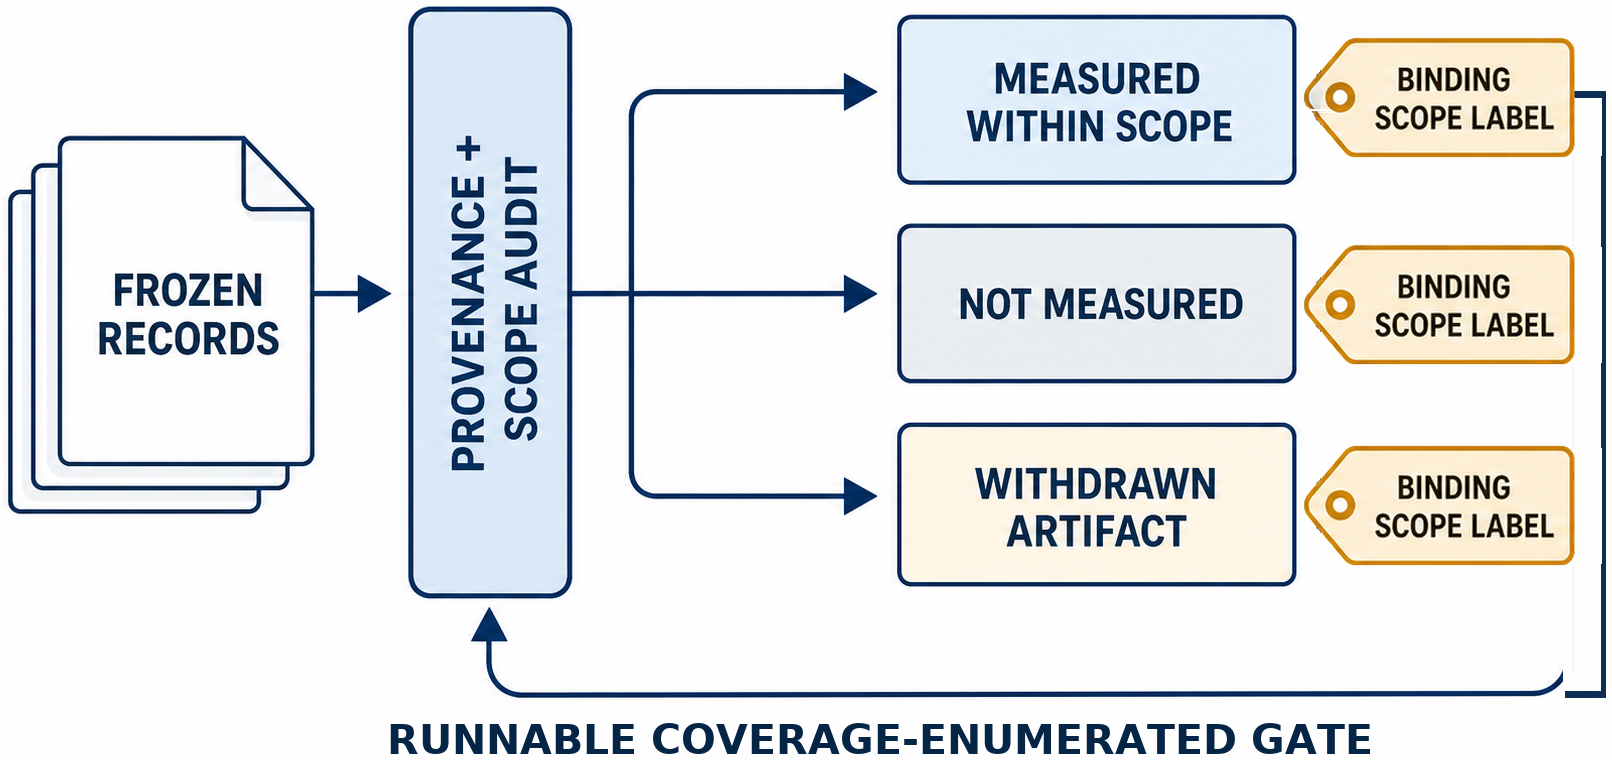
\includegraphics[width=\linewidth]{figures/fig_register_gate_r270.png}
  \caption{The three instruments this note contributes, and how they compose. Frozen records
  pass one provenance-and-scope audit that assigns exactly one of three dispositions; each
  disposition travels with a scope label documenting how the value may be cited; and a
  runnable, coverage-enumerated (pattern-scoped) gate re-checks the manuscript itself against that
  discipline (Section~\ref{sec:p01}). The diagram is methodological and contains no
  quantitative evidence.}
  \label{fig:register-gate}
\end{figure}

\begin{table}[t]
\centering
\caption{Core notation. Arm names describe \emph{where} a query's context is reconstructed
from; the full ledger-ID glossary is Table~\ref{tab:notation-full} in
Appendix~\ref{app:notation}.}
\label{tab:notation}
\footnotesize
\setlength{\tabcolsep}{3pt}
\begin{tabular}{@{}>{\raggedright\arraybackslash}p{1.7cm}>{\raggedright\arraybackslash}p{11.7cm}@{}}
\toprule
\textbf{Term} & \textbf{Definition} \\
\midrule
CoMem & The archived cached-memory serving system; cached arm. \\
$j0$ ($j{=}0$) & The \emph{full-depth} arm: nothing cached; selected chunks replay all layers. \\
$j12$ & The flagship \emph{cached} arm ($j{=}12$ states $+$ LoRA \citep{hu2022lora}). \\
B-only & The full-context dense baseline \emph{without} the (unrecoverable) LoRA arm; every
staircase cell is B-only. \\
$S$ & Per-query CPU cost of chunk-\emph{selection}; algorithmic estimate, not a frozen-corpus
measurement. \\
$G$ & Concurrency; or the generated length in the archived decode model (as labelled per row). \\
$Q^{*}$ & Break-even query count of the cached arm vs the full-depth arm
(Eq.~\ref{eq:qstar}). \\
C/D/S/R-family IDs & Stable claim IDs of the archived ledger (Table~\ref{tab:reg} and
Appendix~\ref{app:notation}). \\
\bottomrule
\end{tabular}
\end{table}

\section{Related Work and Positioning}\label{sec:related}

\textbf{Measurement and reporting methodology.} The closest prior work is not a serving system
but the literature on how empirical claims should be measured and reported. Systems
benchmarking names how performance results mislead \citep{hoefler2015benchmarking} and how bias
can invert a conclusion drawn from careful experiments \citep{mytkowicz2009wrongdata} --- our
failure mode, since the ``capacity boundary'' was a property of the measurement surface.
Machine learning has adopted budget-aware reporting \citep{dodge2019showyourwork},
reproducibility checklists \citep{pineau2021reproducibility}, artifact evaluation
\citep{krishnamurthi2015repeatability}, and structured documentation templates
\citep{gebru2021datasheets,mitchell2019modelcards}. Two strands bear on a withdrawal note:
pre-registration, which fixes analysis scope before the result is known
\citep{nosek2018preregistration}, and non-replication reporting
\citep{dacrema2019progress,kapoor2023leakage}. Closest in spirit, assurance-case notation (the
Goal Structuring Notation; \citealp{kelly2004gsn}) already makes \emph{undeveloped goals} ---
claims an argument states but does not yet establish --- explicit in a structured tree. That
idea is not new.

\textbf{What a NOT\_MEASURED register adds over a Limitations section.} Given that making
unestablished claims explicit predates this work (GSN~\citep{kelly2004gsn}), the register is a
\emph{narrow, machine-checked instance} of that idea, not a new argument formalism. A Limitations
section is free-form prose, and dropping an item need not trigger any failure;
datasheets and model cards fix the \emph{template}, checklists fix the \emph{questions}. The
register adds three machine-checkable properties (Section~\ref{sec:reg},
Table~\ref{tab:frozen}, Section~\ref{sec:p01}): a \emph{complete inventory relative to a declared
universe}, \emph{per-row binding labels} (concurrency, estimand class, status) that forbid
re-citing a value outside the scope that produced it, and a \emph{machine-checked} scope predicate
a reviewer runs, exiting non-zero on violation.

\textbf{Technical background for the withdrawn study.} For context only, and contributing
nothing here: the archived study sat among IO-aware exact attention
\citep{dao2022flashattention}, token- and page-level KV-cache management
\citep{zhang2023h2o,xiao2024streamingllm,adnan2024keyformer,kwon2023pagedattention,ge2024fastgen},
and length-scaled long-context quality probes \citep{hsieh2024ruler,li2023longeval}; its
statistics use the exact conditional paired test \citep{mcnemar1947}, percentile bootstrap
\citep{efron1993bootstrap} and Wilson \citep{wilson1927interval} intervals. The memory-inflation
behind the withdrawal is autograd bookkeeping: outside an inference-mode guard the framework
retains per-layer activations for a backward pass that never happens \citep{paszke2019pytorch}.

\section{Adjudicated Boundaries and Their Enumerated (Pattern-Scoped) Checks}\label{sec:bound}

\subsection{Serial-ledger decoupling is scoped, and the scope is machine-checked}\label{sec:p01}
The same-term cancellation in the archived cost accounting applies to the \textbf{serial
ledger} only, and we make \textbf{zero} wall-clock or concurrency-cancellation claim from that
scoping. The only concurrent wall-clock ever measured on this stack (full-context, no adapter
and no selector; Section~\ref{sec:d1}) carries no selection-cost $S$ term, so there is no
concurrent critical path on which an $S$-cancellation could be asserted; the $S$-removal is
licensed \textbf{only} as a serial-ledger same-term cancellation ($S_0{=}S_c$ on both
serial-ledger sides). A reviewer re-runs the enumerated scope audit
\code{python3 bundle/scanners/\zb audit\_p0\_1\_\zb critical\_path\_scope.py -{}-note bundle/note/main.tex}
(0 GPU, standard library only); it exits 0 only when all four gates hold. The predicates, as
implemented post-\texttt{D1}, with their arm restrictions:

\begin{itemize}\itemsep0pt\parskip0pt
  \item \textbf{G1 (required).} An explicit serial-ledger-only scoping statement is present,
        matched on the literal tokens \code{serial-ledger}, \code{serial ledger}, or
        \code{same-term cancellation}.
  \item \textbf{G2 (required, arm-restricted).} A concurrent-serving NOT\_MEASURED declaration
        is present, matched on \code{not\_measured}, \code{not measured}, or
        \code{unmeasured}. Post-\texttt{D1} that declaration is \emph{arm-restricted}: it governs
        the KV-selector ($j0$) arm, the adapter-matched arm and the $16$k full-context arm, and
        \textbf{not} the full-context arm at $L{=}32$k, which Table~\ref{tab:reg} declares
        MEASURED. The gate checks such a declaration exists, not that every arm is unmeasured, so
        the two statements are consistent.
  \item \textbf{G3 (required).} The withdrawn reading is not re-asserted: four phrase patterns
        are banned in non-negated sentences, including
        \code{permanent (memory|capacity|hardware) bound} and \code{verified in code}. The
        script's original docstring also required the re-attribution to be called
        \emph{suspected}; that gloss is superseded because \texttt{D1} measured it at $32$k. The
        implemented predicate is unchanged.
  \item \textbf{G4 (banned).} No concurrent-critical-path $S$-cancellation claim and no
        concurrency-throughput reading appears, matched against a published enumeration of
        eleven phrase patterns in non-negated sentences.
\end{itemize}

The gate has two published limits. First, it enumerates phrasings: an earlier revision passed
G4 while a throughput-style reading sat in prose outside the enumeration; that reading was
removed, the enumeration extended, and the failure kept as a runnable red-team fixture
(\code{bundle/scanners/redteam/}) so a reviewer confirms the gate now rejects it. Second,
\emph{verbatim \code{code} spans are exempt} from matching --- which is what lets this section
print the banned literals as specification, not assertion; prose is never exempt, so no enumerated
place within the declared phrasing universe remains to hide a claim. A reviewer who finds another
uncovered phrasing has falsified the gate's coverage, not merely disagreed. Bounded by its
enumeration, the gate is falsifiable exactly because it is.

\subsection{The machine-check is a transcript, not a slogan}\label{sec:transcript}
``Machine-checked'' is a concrete run, not a prose promise: Table~\ref{tab:transcript} in
Appendix~\ref{app:transcript} lists every scanner that shipped with this note, what it targets,
the exit code on the frozen text at compile time, the counts it emits, and --- for the scope and
register gates --- a red-team fixture that must {\em fail}, proving the check has discriminative
power rather than always passing. A reviewer re-runs any row against \code{bundle/} (0 GPU,
stdlib only).

\subsection{Adapter identity is partial and provisional}\label{sec:p02}
The shared-flagship-LoRA arm identity was \textbf{provisional}: the declared matched adapter
(\code{dd09cd17\ldots0536f}) could not be retrieved or reproduced, so any dependent
specialization claim is provisional. Two facts are separated so each is independently
verifiable. \textbf{FACT-A}, the measured serving record's own manifest is authentic:
\code{sha256sum -c SHA256SUMS.txt} run \emph{inside} \code{bundle/p1\_8\_serving/} reproduces
\textbf{24/24 files OK} in seconds --- the record's original manifest, a different file from the
bundle-wide \code{bundle/SHA256SUMS.txt} that covers every other shipped artifact.
\textbf{FACT-B}, the adapter weights are not recoverable: zero LoRA weight files
(\code{.safetensors}, \code{.bin}, \code{.pt}) exist anywhere in the bounded release tree, and
\code{dd09cd17} is governed by a withdrawn disposition. FACT-A does not imply FACT-B's negation:
an authentic record of a run is not a recoverable copy of the weights that ran. This note
therefore claims \textbf{no} verified adapter-dependent specialization; re-run
\code{python3 bundle/scanners/\zb verify\_p0\_2\_\zb adapter\_provenance.py -{}-bundle bundle/}
to confirm both.

\subsection{LongEval is direction-only}\label{sec:p04}
On the LongEval line-retrieval suite \citep{li2023longeval}, per-cell Wilson $95\%$ intervals
\citep{wilson1927interval} separate in the same direction at every tested length. But
\textbf{no paired test is claimed and no LongEval value is citable from this note}: per-item raw
outputs were never retained, so the archived pooled statistic is a descriptive comparison between
independent aggregates, not a paired significance result on matched items. The paired re-run is
register row \texttt{D6} of Table~\ref{tab:reg}; until it exists, the LongEval evidence is
directional only.

\section{The NOT\_MEASURED Register}\label{sec:reg}
Table~\ref{tab:reg} is the register, and \textbf{its universe is declared, not rhetorical}: the
rows enumerate the load-bearing claims of the archived claim ledger at closure --- the C-numbered
serving/quality claims, D-numbered decisive-evidence debts, and S-numbered soundness-deficit
classes. Completeness is asserted \emph{relative to that enumerable, shipped ledger}, not to every
statement a reader might form, and is falsified by exhibiting a ledger item with no row. The limit
is that the ledger is \emph{author-constructed}: the register certifies no \emph{ledgered} claim
lacks a row, but cannot prove none was ever omitted (third-party recovery is the narrowing check
we have not run); and the exact-set \emph{semantic} check is clue-scoped, not a general
guarantee --- each registered ID appears and every canonical semantic clue in the text after it
belongs to that same ID (a swap that moves one ID's meaning onto another's row is caught by the
shipped mutation fixture), but a substitution borrowing no canonical clue, or one outside the
per-ID text window, is unseen. A new failing mutation falsifies one of these bounds, as the
red-team fixtures do.

\textbf{Exact-set completeness is machine-checked.} Table~\ref{tab:reg} is \emph{generated}
from the checked-in single source \code{tools/register\_ledger\_check.py} (LEDGER + REGISTER +
DECLARED\_MERGES), and every row carries an explicit \textbf{Ledger-ID} column that spans the
full C/D/S closure universe: C-numbered claims retained, D-numbered decisive-evidence debts,
S-numbered soundness-deficit classes. The generator and the checker enforce the same
invariants --- every ledger ID has a row, no row adds an unknown ID, and any many-to-one merge
(e.g.\ $S1{/}S3{/}S6 \rightarrow$ one row) is declared and counted --- so deleting a row (e.g.\
omitting \texttt{D4}) or diverging a status canonical token makes the build fail non-zero,
rather than silently passing (Section~\ref{sec:p01}).

\begin{table}[tp]
\centering
\caption{The NOT\_MEASURED register, machine-generated from the checked-in single source
(\code{tools/register\_ledger\_check.py}). Each row binds Ledger-ID entries --- spanning the
C (claim retained), D (decisive-evidence debt) and S (soundness-deficit) families --- to their
arm and scope, canonical status, and closing measurement. Statuses come from one vocabulary
shared with Table~\ref{tab:frozen}: \texttt{MEASURED}, \texttt{DERIVED}, \texttt{ESTIMATE}
(algorithmic, not measured), \texttt{EXTRAPOLATED} (outside the measured range),
\texttt{NOT\_MEASURED}, \texttt{CLOSED\_WRITING} (closed by a writing-only declaration, not
empirically), \texttt{NOT\_ADJUDICATED} (reported for completeness, not citable as a
prediction). The last two are printed because the checker fixes the vocabulary, not this table;
no row here carries them. The \texttt{D4} row and the $S1{/}S3{/}S6$ merged row instantiate the
many-to-one semantic formalization.}
\label{tab:reg}
\footnotesize
% R270 (audit item B12): the 12 rows are machine-generated and must stay byte-identical to
% tools/gen_register_tables.py, so row-group spacing cannot be added inside them. \extrarowheight
% buys the same visual separation from outside the row bodies, leaving every row untouched.
\setlength{\extrarowheight}{1pt}
\setlength{\tabcolsep}{1.5pt}
\begin{tabular}{@{}>{\raggedright\arraybackslash}p{1.35cm}>{\raggedright\arraybackslash}p{3.3cm}>{\raggedright\arraybackslash}p{2.15cm}>{\raggedright\arraybackslash}p{2.8cm}>{\raggedright\arraybackslash}p{3.85cm}@{}}
\toprule
\textbf{Ledger ID} & \textbf{Ledger item} & \textbf{Arm / scope} &
\textbf{Status} & \textbf{What would close it} \\
\midrule
C4 & serial-cost ledger: CoMem/j0 serving cost terms & family C; serial cost & MEASURED & MEASURED from frozen 24-file manifest (\code{p1\_8\_serving}); citable within serial-cost scope \\
C7 & memory slope vs time-power-law exponent (B-only capacity staircase) & family C; serial capacity; $G{=}1$ & DERIVED & co-measured memory and prefill-time record at the same operating point \\
C9 & RULER macro accuracy gap and bootstrap & family C; quality; macro over 15 cells & DERIVED & item-level paired McNemar on the retained raw outputs \\
C13 & $Q^{*}$ crossover estimate class & family C; serial cost; crossover & ESTIMATE & measured per-query margin at $G{=}1$ (not an estimate) \\
D1 & concurrent full-context serving @ $L{=}32$k (grad-mode fix-and-rerun) & family D; full-context; concurrent $G{\in}\{1,4\}$; $L{=}32$k & MEASURED & MEASURED (\texttt{D1} fix-and-rerun at $L{=}32$k, no OOM; Table\,\ref{tab:d1}; throttle curve remains open) \\
D1-16k & concurrent full-context serving @ $L{=}16$k re-run & family D; full-context; $L{=}16$k & NOT\_MEASURED & NOT\_MEASURED: re-run the guarded full-context arm at $L{=}16$k; the current $16$k peak is inspection-grade cross-scope reference only (Section\,\ref{sec:d1}) \\
D2 & adapter-source recovery / rebuild & family D; adapter; serial and concurrent & NOT\_MEASURED & recover or rebuild the declared adapter, then re-run \\
D3 & KV-selector ($j0$) finite fetch & family D; selector; concurrent & NOT\_MEASURED & repair \code{create\_causal\_mask} argument mismatch (three call sites), then re-run \\
D4 & adapter-identity table completeness & family D; adapter; writing declaration & CLOSED\_WRITING & CLOSED\_WRITING: closed by a writing-only declaration, not empirically (this table) --- completeness is relative to the enumerated ledger \\
D5 & adapter-identity per-row binding caveat & family D; adapter; per-row scope & CLOSED\_WRITING & CLOSED\_WRITING: every identity value carries a per-row binding caveat (this table), not a verified equality \\
D6 & LongEval per-item (paired) re-run & family D; quality; LongEval; direction-only currently & NOT\_MEASURED & retain per-item outputs and run paired McNemar; needs GPU and a scorer environment \\
S1/S3/S6 & single-arm isolation of the scoped mechanism & family S; any arm; serial & NOT\_MEASURED & single-arm run with co-measured cost and quality \\
\bottomrule
\end{tabular}
\end{table}

\textbf{One cross-scope reference, labelled as such.} The guarded \emph{serial} staircase
records $22.30$\,GB at $16$k (C7, serial ledger, $G{=}1$; Table~\ref{tab:frozen}). For the
\texttt{D1-16k} row of Table~\ref{tab:reg} that value is a \textbf{serial cross-scope reference}, not a concurrent
measurement of it and not an independent confirmation of it. Its role is bounded and stated in
Section~\ref{sec:d1}: same model, dtype, attention backend and GPU as the pre-guard concurrent
$16$k observation, hence a same-hardware comparison point for the guard mechanism.

\section{Frozen Measurable Values, With Per-Row Binding Scope}\label{sec:frozen}
The values in Table~\ref{tab:frozen} are citable \textbf{only} with the scope printed on their
own row. There is no table-wide scope, because the rows are heterogeneous by design: C13's
replicate row is a $G{=}512$ figure, not a $G{=}1$ serial one, and C9's rows are accuracy
estimands, not cost figures. An earlier version carried a universal ``every value is a serial
$G{=}1$ figure'' preamble that its own C13 row falsified. Rows must not be combined into a
serving$\times$quality metric.

\begin{table}[t]
\centering
\caption{Frozen measurable values with per-row binding scope. ``$G$'' is the row's concurrency
or generated-length setting ($-$ where concurrency does not apply, as for accuracy estimands).
Status tokens are the canonical vocabulary of Table~\ref{tab:reg}: \texttt{MEASURED} (read from a
frozen record), \texttt{DERIVED} (computed from measured values by the stated estimator),
\texttt{ESTIMATE} (algorithmic only), \texttt{NOT\_ADJUDICATED} (reported for completeness, not
citable as a prediction). Rows are grouped by claim family. No cross-row aggregation and no
concurrent-serving inference is licensed by any row.}
\label{tab:frozen}
\footnotesize
% R270 (audit item B12): the status column is 2.7cm so the canonical token NOT_ADJUDICATED
% (84pt at this size) sets as one word instead of being split at its underscore; the room comes
% from the quantity column and from the column separation, both of which had slack: the longest
% quantity entry already wrapped at a space either way, so no row gains a line.
\setlength{\tabcolsep}{1.5pt}
\begin{tabular}{@{}>{\raggedright\arraybackslash}p{0.7cm}>{\raggedright\arraybackslash}p{3.7cm}>{\raggedright\arraybackslash}p{3.3cm}c>{\raggedright\arraybackslash}p{2.15cm}>{\raggedright\arraybackslash}p{3.05cm}@{}}
\toprule
\textbf{ID} & \textbf{Quantity} & \textbf{Value (units)} & \textbf{$G$} &
\textbf{Estimand class} & \textbf{Status} \\
\midrule
C4 & CoMem write @128k, one-time & $6.65$\,s & 1 & serial cost & MEASURED \\
C4 & $j0$ index build @128k, one-time & $0.022$\,s & 1 & serial cost & MEASURED \\
C4 & CoMem cache read, per query & $0.68$\,s/q & 1 & serial cost & MEASURED \\
C4 & $j0$ read, per query & $0.94$\,s/q & 1 & serial cost & MEASURED \\
C4 & fetch, per query (CoMem / $j0$) & $0.0014$ / $0.00002$\,s/q & 1 & serial cost & MEASURED \\
\addlinespace
C7 & B-only full-context peak at $8$/$16$/$32$/$64$/$128$k
   & \mbox{$18.80$/$22.30$/$29.31$/}\allowbreak\mbox{$43.34$/$71.38$\,GB} & 1 & serial capacity & MEASURED \\
C7 & B-only cache peak @128k & $18.29$\,GB & 1 & serial capacity & MEASURED \\
C7 & full-context prefill time at $8$/$16$/$32$/$64$/$128$k
   & \mbox{$1.28$/$2.98$/$7.75$/}\allowbreak\mbox{$22.26$/$72.74$\,s} & 1 & serial cost & MEASURED \\
C7 & growth exponent of prefill time in $L$ & $1.46$ (dimensionless) & 1
   & serial fit, 5 points & DERIVED \\
\addlinespace
C9 & RULER macro accuracy gap & $3.12$\,pp & $-$ & quality, macro over 15 cells & MEASURED \\
C9 & cell-level $95\%$ percentile bootstrap CI & $[1.69,\,4.68]$\,pp & $-$
   & quality, cell level & DERIVED \\
C9 & item-level discordant counts $b$/$c$/$n$ & $83$ / $1$ / $84$ & $-$
   & quality, pooled item level & MEASURED \\
C9 & exact two-sided McNemar $p$ & $8.79{\times}10^{-24}$ & $-$
   & quality, pooled item level & DERIVED \\
C9 & pooled accuracy gap & $5.47$\,pp & $-$ & quality, pooled & MEASURED \\
\addlinespace
C13 & paired per-query margin @128k & $0.0404$\,s/q & 512
    & crossover input & MEASURED \\
C13 & $Q^{*}$ @$128$k (aggregate grid) & $25.8$\,queries & 1
    & crossover, model-implied: Eq.~\ref{eq:qstar} with inputs in Table~\ref{tab:qstar} & DERIVED \\
C13 & $Q^{*}$ @$32$k & $8.4$\,queries & 1
    & crossover, model-implied: Eq.~\ref{eq:qstar}; inputs not separately printed & DERIVED \\
C13 & $Q^{*}$ @$1$M & $180.2$\,queries & 1
    & crossover beyond the measured staircase ($\le 128$k); model-implied & EXTRAPOLATED \\
C13 & $Q^{*}$ @128k, replicate & $164.2$\,queries & 512
    & crossover, replicate & DERIVED \\
\addlinespace
R142 & full-context write model $W(L)$
     & $4.432{\times}10^{-5}L$ $+\,0.775$\,s & 1 & in-sample fit, 3 points
     & NOT\_ADJUDICATED \\
\bottomrule
\end{tabular}
\end{table}

\textbf{Estimators, so every derived row is reproducible from the printed inputs.}
\begin{itemize}\itemsep0pt\parskip0pt
  \item \textbf{C9.} On the discordant counts $b$/$c$/$n$ printed in Table~\ref{tab:frozen}, the
        two-sided exact conditional McNemar test gives
        $p = 2\sum_{k=0}^{\min(b,c)}\binom{n}{k}2^{-n}$, so those counts alone reproduce the
        printed $p$. That test is at the \emph{pooled item level}, whereas the interval is a
        percentile bootstrap at the \emph{cell level} (15 RULER cells, seed 123,
        $n_{\mathrm{boot}}{=}20000$) around the macro gap. \textbf{No test is claimed for the
        macro gap}, and the pooled gap is a same-direction but distinct estimand rather than a
        second estimate of it. Figure~\ref{fig:ci} (Appendix~\ref{app:ci}) plots the two
        intervals this note cites; neither includes zero.
  \item \textbf{C13.} With per-query cost
        $c_{\mathrm{arm}}(G)=\mathrm{fetch}+\mathrm{read}+\mathrm{decode}(G)$,
        \begin{equation}\label{eq:qstar}
          Q^{*}(L)\;=\;\frac{W_{\mathrm{CoMem}}(L)-I_{j0}(L)}
                            {\overline{c_{j0}(G)-c_{\mathrm{CoMem}}(G)}}.
        \end{equation}
        The numerator differences the two \emph{one-time} costs; the denominator is the mean
        paired per-query margin, defined only where positive. $Q^{*}$ grows with $G$ because
        decode does \emph{not} cancel between the arms, so its values at two concurrency
        settings are \emph{different quantities} rather than a contradiction; and $S$ does
        \emph{not} enter Eq.~\ref{eq:qstar}, so every input is measured.
        \mbox{Table~\ref{tab:qstar}} (Appendix~\ref{app:derived}) carries the inputs, the
        quotients and the per-row provenance flag, including the superseded face whose
        denominator is not reproducible from the printed components.
  \item \textbf{C7.} The three slopes of Table~\ref{tab:derived}
        (Appendix~\ref{app:derived}) are \emph{different
        quantities} and must not be interchanged: $1.46$ is the least-squares slope of
        $\log t$ on $\log L$ over the five \emph{prefill times}; the same estimator on the
        \emph{peak-memory} series gives $0.48$, and peak memory is near-affine in $L$ at
        $0.438$\,GB\,per\,$1$k tokens.
  \item \textbf{$S$ versus C4's selection-side terms: different quantities, not a discrepancy.}
        $S$ is the \emph{per-query} CPU cost of scoring chunks (Table~\ref{tab:derived}),
        an algorithmic estimate on representative chunks rather than the frozen corpus.
        C4's ``$j0$ index build'' ($0.022$\,s @128k) is the \emph{one-time} $O(L)$ index
        construction over the whole store, entering Eq.~\ref{eq:qstar}'s numerator beside the
        one-time write rather than any per-query term; C4's ``$j0$ read'' ($0.94$\,s/q) is the
        per-query 36-layer replay. The three sit at different decomposition granularity and are
        not expected to reconcile numerically; Figure~\ref{fig:profiles} (right) shows the split.
\end{itemize}

\begin{figure}[t]
  \centering
  % Authored at \textwidth (5.5in) and printed 1:1, so the artwork's 8pt labels print at 8pt.
  % The previous two-minipage layout printed 4.7in panels at 2.34in, which is why the R174
  % audit read the panel text as too small; the plotted values are unchanged.
  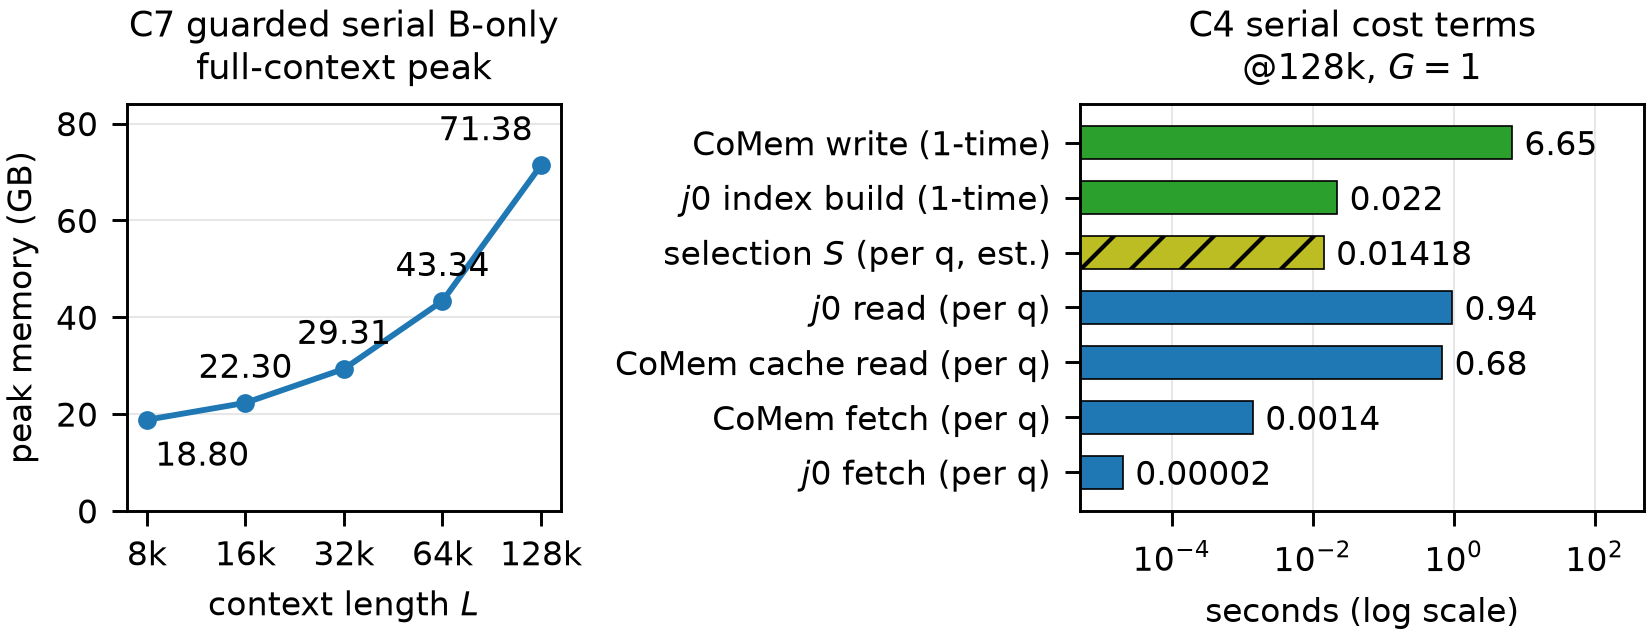
\includegraphics[width=\linewidth]{figures/fig_serial_profiles_r176.png}
  \caption{Frozen serial-ledger profiles, plotted from the bundled datacards behind
  Table~\ref{tab:frozen}. \textbf{Left:} guarded B-only full-context peak memory rises
  monotonically with context length (\code{bundle/staircase/\zb fullctx\_serving.json}); this is
  the guarded serial surface, and the pre-guard concurrent observations of Section~\ref{sec:d1}
  are not on it. \textbf{Right:} the @128k, $G{=}1$ cost terms on a log axis, split into one-time
  and per-query classes, the hatched bar being the unmeasured algorithmic estimate $S$; each tick
  label carries its class, \mbox{(1-time)} for a cost paid once per store and \mbox{(per q)} for
  one paid per query. The log
  axis is needed because the terms span five orders of magnitude, and the one-time/per-query
  split is what keeps the $0.022$\,s index build from being read as a per-query selection cost.
  Both panels are scoped serial references, never concurrent-serving or capacity claims.}
  \label{fig:profiles}
\end{figure}

\section{The D1 Concurrent Fix-and-Rerun, and What It Does Not Cover}\label{sec:d1}

\textbf{Two application-level defects, one fixed and measured, one only diagnosed.} The
concurrent experiment was previously reported as blocked by the environment; static audit of our
own measurement code found two defects with different evidential status instead. (i) A
\emph{thread-local grad-mode leak}: the concurrent worker called the model outside any
\code{torch.inference\_mode()}/\code{no\_grad()} scope that the serial baseline wrapped the same
forward in. Because grad mode is thread-local, worker threads inherited autograd \emph{on} and
retained 36 layers of activations for a backward pass that never occurs
\citep{paszke2019pytorch}. The repair is $\approx$2 lines and \textbf{has been applied and
re-measured}. (ii) A \emph{framework-version argument mismatch}: the vendored QCMem selector
calls \code{create\_causal\_mask} with keyword \code{inputs\_embeds}, whereas installed
\code{transformers} 4.54.1 names that parameter \code{input\_embeds}; the $\approx$6--10-line
repair across three call sites needs no \code{transformers}${\ge}$5.5 upgrade but is
\textbf{statically diagnosed only, not re-measured}. The two stay separate rather than being
summed into one ``$\approx$10-line'' blocker, because only the first is backed by a measurement.

\textbf{What D1 measured.} After the guard, the full-context arm at $L{=}32$k runs end to end
at both tested concurrency levels, with finite decode and no out-of-memory failure; every value
is on its own row of Table~\ref{tab:d1}, and the matched pair is \emph{pre-guard abort} versus a
\emph{post-guard finite peak}. Two scope labels attach to the two pre-guard rows of that table.
First, the pre-guard $32$k job recorded \textbf{no peak} before aborting, so the tensor-size
figure sometimes attached to $32$k is \emph{analytical}, from a superseded root-cause account,
and never a measured peak. Second, the pre-guard $16$k job \emph{did} record a peak, on the same
model, dtype, attention backend and GPU as the guarded serial surface --- consistent with
activations retained across all 36 layers. That $16$k comparison is \emph{inspection-grade}: no
$16$k concurrent re-run was produced, so the $16$k row stays NOT\_MEASURED
(Table~\ref{tab:reg}), even though its peak is a measured record. The earlier reading of D1 as a
memory or infeasibility \emph{boundary} is therefore withdrawn --- at $32$k the full-context
concurrent state is feasible and the inflation was a property of our measurement code --- while
the KV-selector arm, the adapter-matched arm and the $16$k re-run remain unmeasured. D1 closes
exactly one register row.

\begin{table}[t]
\centering
\caption{The D1 concurrent full-context measurement at $L{=}32$k, after the two-line
inference-mode guard. Single H20-3e (141\,GB), Qwen3-8B \texttt{bfloat16}, SDPA attention,
store $L{=}32$k, read sample $8$k, task \code{niah\_multikey\_1}, 8 queries, $R{=}3$ rounds,
seed 42, no adapter, no selector. Wall-clock is \emph{per request} and includes queue wait
under contention. Dispersion is the coefficient of variation, which is what the driver
retained. Source \code{bundle/d1/\zb e2e\_concurrent\_kvsel.json}; applied diff
\code{bundle/d1/D1\_FIX.diff}.}
\label{tab:d1}
\small
\begin{tabular}{@{}ccccc>{\raggedright\arraybackslash}p{4.6cm}@{}}
\toprule
\textbf{$G$} & \textbf{Peak (GB)} & \textbf{Median (s)} & \textbf{CV} &
\textbf{$n$ ($R{\times}G$)} & \textbf{Role of this row} \\
\midrule
$1$ & $29.31$ & $7.71$ & $0.031$ & $3=3{\times}1$ & consistency check (see below) \\
$4$ & $70.73$ & $30.63$ & $0.001$ & $12=3{\times}4$ & the concurrency datum \\
\midrule
pre\--guard $32$k & none (abort) & --- & --- & $1$ & no peak recorded; the $137.4$\,GB figure is analytical only, never measured \\
pre\--guard $16$k & $139.2$ & --- & --- & $1$ & cross-scope reference, inspection-grade vs serial $22.30$\,GB (see text) \\
\bottomrule
\end{tabular}
\end{table}

\textbf{Replication structure, stated rather than implied.} The $n$ column counts
\emph{per-request} samples: $n{=}12$ at $G{=}4$ is 3 rounds of 4 simultaneous requests sharing a
queue and a device, so the effective independent replication is \textbf{3 rounds per level}. The
driver retained only median, CV and $n$; per-request wall-clocks were not persisted, so an IQR or
range is not recoverable from the frozen record, and we do not manufacture one.

\textbf{The $G{=}1$ row is a consistency check, not a second concurrency datum.} At $G{=}1$ the
driver submits one in-flight request through the same full-context forward path as the serial
staircase: its peak equals the serial C7 $32$k entry of Table~\ref{tab:frozen} exactly, and its
median wall-clock agrees with the serial read time to within $0.6\%$. We read this as
cross-surface agreement that the guarded surface is the same surface --- \textbf{not} an
independent second concurrency level; the withdrawal's concurrency content rests on the $G{=}4$
row alone.

\textbf{No throughput reading is offered.} The two rows are peak-feasibility and wall-clock
records. The $G{=}4$ to $G{=}1$ median ratio is $\approx 4$, but with one reference
implementation, one operating point per level, 3 effective replicates and no controlled
contention arm, the ratio identifies no mechanism; we make \textbf{no} concurrency-throughput,
latency or scalability claim (a prior version printed the ratio at three significant figures and
glossed it as a throughput result; that reading is removed, not re-disclaimed).

\textbf{Quality debt carried forward (D2--D6, S1).} D2, adapter source recovery, is an external
artifact-access problem rather than a code fix. D6, the LongEval per-item re-run, needs GPU and a
scorer environment. D4, adapter identity in the archived tables, is closed here as a writing-only
declaration (Section~\ref{sec:p02}). S1, single-arm isolation, needs GPU; D3, the KV-selector
($j0$) finite fetch, is statically diagnosed but not re-measured.

\textbf{Environment-boundary honesty.} No failure was retried to burn: every failing job was
stopped and reported, and all GPU consumption is in the shipped burn ledger (cumulative
$1.82$\,GPU$\cdot$h, ``0 data'' across five fires). The driving code logs
\code{torch.cuda.max\_memory\_allocated()} before failing, so a pre-guard peak exists at $16$k; the
earlier $32$k job predates that logging, which is why none exists there.

\section{Consumption Discipline (Binding on Re-Use)}\label{sec:discipline}
The following are required interpretations for any later text that re-uses values from this note;
they are prohibitions on inference, not on discussion.
\begin{itemize}\itemsep0pt\parskip0pt
  \item \textbf{Do not} re-assert ``selection is cheap or $S$-symmetric, therefore concurrent
        wall-clock cancels'': no concurrent selector critical path was ever measured.
  \item \textbf{Do not} read the LongEval gap as a paired significance result, and do not claim
        adapter-arm identity is verified.
  \item \textbf{Do not} read Table~\ref{tab:d1} as throughput, scalability or latency.
  \item Cite frozen values only with the scope printed on their own row
        (Table~\ref{tab:frozen}): no derived extrapolation, no combined
        serving$\times$quality metric.
  \item Report failures loudly; do not re-fire a failed job to consume budget.
\end{itemize}

\section{Method Validity: Cross-Case Transfer}\label{sec:method}
The instrument is not a description of this one withdrawal case: the read-only six-family
scanner (\code{bundle/method/\zb independent\_claim\_audit.py}, 0 GPU) also ran on an
\textbf{independent project} --- the S1 SparseForge manuscript (934 lines, a different group's
paper, different area) --- striking \textbf{91 signal hits} across all six families
(\code{audit\_sparseforge.json}) under a different, \emph{provenance-crisis-led} honesty
structure. The same tool yields 68 hits on this note (withdrawal-dense, 28 WITHDRAWN), so the
scan distinguishes failure-mode \emph{structures}, not a ``more hedging $=$ more honest''
counter; the per-family split of both runs is the last row of
Table~\ref{tab:transcript} (Appendix~\ref{app:transcript}).

The transfer shows the \emph{scan} generalizes, not that any downstream evaluation score is
comparable across projects. Two validity checks are reported in
Appendix~\ref{app:validity}: an \emph{independent-annotator} recovery study (a reader blind to
our ledger recovered all 14 register IDs at the paper's semantics) and a
\emph{coverage-self-critique} of the six-family taxonomy, which is \textbf{not exhaustive} ---
the scanner is a \emph{necessary} hygiene filter, not a complete-honesty certificate.

\textbf{Layout step-width is NOT\_MEASURED on held-out partitions.} The mechanical
formatting/layout revisions in this note's history (float placement, collapse to the 9-page
main-text limit, caption and font scaling) are \texttt{NOT\_MEASURED} improvements: none was
re-verified on an un-measured/held-out visual partition by an independent layout audit at every
step. We claim only that the artifact's content and scope gates hold; the layout step-width is
not a measured gain and must not be cited as one until an independent visual audit passes on a
frozen face.

\section{Conclusion}\label{sec:concl}
The guarded rerun shows that the full-context arm at $L{=}32$k is feasible at both tested
concurrency levels, with finite decode and no out-of-memory failure
(Table~\ref{tab:d1}).  This establishes that the earlier apparent environment or hardware
boundary was, at that length, a measurement-code defect.  The frozen serial values remain
citable only within their row-specific scopes.  The KV-selector arm, adapter-matched arm,
and guarded $16$k concurrent rerun remain unmeasured; the $16$k attribution is
inspection-grade, and the $G{=}4$ row is the sole concurrency datum, with 3 effective
replicates.  The contribution is therefore a reporting instrument rather than a serving
result: a declared-ledger register, per-row scope labels, and an enumerated pattern-scoped
gate whose uncovered phrasing remains criticizable.  The instrument applies only where an
enumerable claim ledger exists and cannot replace the missing measurements; it makes their
status auditable within this record.

% P5_MAIN_TEXT_END
\label{p5:main-text-end}
%% Give the two-page reference block one extra line on the page it starts so
%% the final entry does not spill a lone line onto a near-empty trailing page.
\enlargethispage{2\baselineskip}
{\small
\setlength{\bibsep}{0pt}
\bibliographystyle{iclr2026_conference}
\bibliography{refs}
}

% R270 (audit items A1/A2): the four supporting objects below used to be declared in the main
% text, where the register table's own height meant none of them could be placed as a top float;
% LaTeX honours float order, so they queued and were flushed by the final \clearpage, printing
% four to seven pages after their citation and leaving one page ~70% empty. Each now sits in its
% own appendix section under a title the reader can see, anchored with [H] so it prints exactly
% where it is declared and cannot drift from its section again.
\appendix

\section{Reproducibility and Ethics Statements}\label{sec:repro}
{\footnotesize
Every value citable in this note is verifiable against a shipped frozen record (checkable, in
\code{bundle/} with \code{SHA256SUMS.txt} and per-item READMEs), and most derived quantities
re-compute from their printed inputs with 0 GPU and only the standard library. Not every
recovered artifact is end-to-end re-runnable --- the declared adapter and the LongEval per-item
outputs are unrecoverable --- so ``runtime'' is not claimed where it does not hold. The note
source is bundled at
\code{bundle/note/main.tex} so the scope gate can run against the frozen text itself.

\textbf{Artifact verification.} An anonymized archive of \code{bundle/} (with its
\code{SHA256SUMS.txt} and per-item READMEs) ships at the link on this manuscript's blind
submission; no artifact path here is specific to any author identity. A reviewer verifies the
retrieved bytes by digest: the bundle manifest \code{SHA256SUMS.txt} has
\texttt{\zb dfa477175acb79497e59a0de7c3aad9de72bd72d2c30ba99f050d196d9567322 \zb}
and \code{sha256sum -c SHA256SUMS.txt} inside the retrieved \code{bundle/} reproduces all shipped
artifacts --- including the manuscript source \code{bundle/note/main.tex} that the scanner
registers (Section~\ref{sec:p01}, Section~\ref{sec:reg}) run against. The compiled PDF is
produced deterministically from that source, so its digest is recorded in this revision's build
receipt and re-derived by recompiling; a reviewer needs only the standard library and 0 GPU.
% These bullets are mostly unbreakable \code{} paths; justifying them stretched interword
% space to badness 10000 on several lines, so this one list is set ragged-right.
\begin{itemize}\itemsep0pt\parskip0pt\raggedright
  \item \textbf{Scanners} (G1--G4 scope, adapter provenance, grad-mode, register): see the
        transcript in Table~\ref{tab:transcript} (Appendix~\ref{app:transcript}) and
        Section~\ref{sec:p01}.
  \item \textbf{D1 measurement} (Table~\ref{tab:d1}):
        \code{bundle/d1/\zb e2e\_concurrent\_kvsel.json}, applied diff
        \code{bundle/d1/D1\_FIX.diff}, gate verdict \code{bundle/d1/\zb feas\_verdict.json};
        pre-guard evidence \code{bundle/oom/\zb fullctx\_16k\_oom.log} ($139.2$\,GB recorded) and
        \code{bundle/oom/\zb fullctx\_32k\_oom.log} (abort) --- records of the pre-fix surface,
        never capacity bounds.
  \item \textbf{Datacards} behind Table~\ref{tab:frozen}:
        \code{bundle/staircase/\zb fullctx\_serving.json} (C7),
        \code{bundle/\zb ruler\_ci\_bootstrap.json} (C9),
        \code{bundle/qstar\_dispersion\_reanalysis.json} (C13; superseded by the aggregate grid),
        \code{bundle/\zb s\_estimate\_iterbm25.json} ($S$), and
        \code{bundle/p1\_8\_serving/} (C4/C13, 24-file manifest).
  \item \textbf{Method-transfer audit}: \code{bundle/method/\zb independent\_claim\_audit.py},
        \code{audit\_sparseforge.json}, \code{audit\_ownnote.json}.
  \item \textbf{GPU accounting}: \code{bundle/burn/HONEST\_BURN\_*.md}.
\end{itemize}
\textbf{Ethics.} This work involves no human subjects, no personal or sensitive data and no
model release. Its only foreseeable risk is misuse of the retained numbers outside their
recorded scope, which Section~\ref{sec:discipline} exists to constrain. The withdrawal of an
earlier interpretation is reported in full rather than silently corrected.
}

\section{Machine-Check Transcript}\label{app:transcript}
Every scanner shipped with this note, with the exit code it returns on the frozen text at compile
time (Section~\ref{sec:transcript}). Paths are relative to the release root, and each scanner's
path heads its own full-width row so that no path is broken across lines.

\begin{table}[!ht]
\centering
\caption{Machine-check transcript: for each scanner, its target, its exit code on the frozen
text, the counts it emits, and its red-team verdict. A fixture that must {\em fail} is what
separates a check with discriminative power from one that always passes; \code{n/a} marks a
structural or same-source check for which a fixture is not the relevant evidence.}
\label{tab:transcript}
\small
\setlength{\tabcolsep}{3pt}
\begin{tabular}{@{}>{\raggedright\arraybackslash}p{3.9cm}c>{\raggedright\arraybackslash}p{4.1cm}>{\raggedright\arraybackslash}p{4.3cm}@{}}
\toprule
\textbf{Target} & \textbf{Exit} & \textbf{Match counts (frozen text)} &
\textbf{Red-team verdict} \\
\midrule
\multicolumn{4}{@{}l}{\code{bundle/scanners/audit\_p0\_1\_critical\_path\_scope.py}} \\
main.tex; G1--G4 scope & 0 &
 G1$=$4, G2$=$3, G3$=$0, G4$=$0 &
 \code{redteam/FIXTURE1} fails (rc$=$1): G4 rejects
 \code{concurrency\zb-throughput} gloss \\
\addlinespace
\multicolumn{4}{@{}l}{\code{bundle/scanners/audit\_grad\_mode\_guard.py}} \\
vendored e2e bench sources & 0 &
 baseline guarded, worker unguarded; fix locus present &
 n/a (structural) \\
\addlinespace
\multicolumn{4}{@{}l}{\code{bundle/scanners/verify\_p0\_2\_adapter\_provenance.py}} \\
bundle; FACT-A/B & 0 &
 FACT-A 24/24 manifest OK; FACT-B 0 weight files &
 n/a \\
\addlinespace
\multicolumn{4}{@{}l}{\code{tools/register\_ledger\_check.py}} \\
registry LEDGER/REGISTER & 0 &
 12 rows exact-set; statuses canonical &
 9 known-bad mutations all {\em fail} \\
\addlinespace
\multicolumn{4}{@{}l}{\code{tools/gen\_register\_tables.py}} \\
main.tex Table~\ref{tab:reg} (same source) & 0 &
 12 rows $=$ registry, no drift &
 n/a (drift vs checker = build fail) \\
\addlinespace
\multicolumn{4}{@{}l}{\code{bundle/method/independent\_claim\_audit.py}} \\
main.tex, six families & 0 &
 68 hits (28 WITHDRAWN / 8 NOT\_MEASURED / 5
 OVERCLAIM\_RISK / 5 HEDGE / 19 PROVENANCE / 3 MATCHED) &
 independent manuscript (S1) 91 hits, distinct
 failure-mode structure \\
\bottomrule
\end{tabular}
\end{table}

\section{Scanner Validity: Independent Recovery and Coverage Self-Critique}\label{app:validity}
Two 0-GPU validity studies (Section~\ref{sec:method}) bound how the six-family scanner may be
read.
\paragraph{Independent-annotator recovery.}
A reviewer blind to our ledger re-extracted the load-bearing claims from the frozen PDF and
recovered all 14 C/D/S register IDs with the same canonical semantics the paper assigns them
(51 claims: 21 MEASURED, 10 NOT\_MEASURED, 7 withdrawal, 5 scope, 5 method-instrument, 3
cross-case; \code{bundle/validity/\zb annotator\_recovery.json}). Its skeptical omissions
were all already-honest disclaimers in the paper (single-point D1 replication; the
author-constructed ledger limit; inspection-grade $16$k attribution); none was a registered
claim absent from the paper.
\paragraph{Coverage self-critique.}
A blind mapping of this note's own prose honesty onto the six families left 9 of 27 structures
outside any family --- the structures that most distinguish the note: an
\emph{attribution-grade} distinction (measured vs.\ \emph{by inspection} vs.\
\emph{analytical-only} vs.\ derived), declared-universe completeness, refusal-to-aggregate
integrity, effective-vs-nominal sample size, and false-precision
(\code{bundle/validity/\zb coverage\_self\_critique.json}). The six families are a
\emph{necessary} hygiene filter: a scanner built purely from them would pass this note's
strongest honesty structures unseen.

\section{\texorpdfstring{$Q^{*}$}{Q*} Reconciliation and the Derived Sequences}\label{app:derived}
The two tables the C13 and C7 estimators of Section~\ref{sec:frozen} point at. Both are read as
rows rather than as prose because every entry is one of a set of comparable quantities.

\begin{table}[!ht]
\centering
\caption{C13 $Q^{*}$ reconciliation at $L{=}128$k. The inputs are the printed per-query
components of \code{bundle/p1\_8\_serving/\zb p1\_8\_serving\_aggregate.json} (cell
\texttt{gpu}); the one-time numerator $W_{\mathrm{CoMem}}{-}I_{j0}$ is shared by every row, so
the rows differ only in their denominator. Each citable row reproduces from the printed inputs.
The superseded face is a replicate-level paired-bootstrap reanalysis
(\code{bundle/\zb qstar\_dispersion\_reanalysis.json}): its denominators are bootstrap means over
replicates and are \emph{not} recomputable from the printed per-query components, which is why the
aggregate grid supersedes it for point values, and its own datacard flags it as not a reproduction
of the frozen $G{=}1$ figure.}
\label{tab:qstar}
\footnotesize
\setlength{\tabcolsep}{4pt}
\begin{tabular}{@{}l l l c l@{}}
\toprule
\textbf{Case} & $W_{\mathrm{CoMem}}{-}I_{j0}$ (s) & \textbf{mean paired margin} (s/q)
 & $Q^{*}$ & \textbf{denominator recomputable} \\
\midrule
\multicolumn{5}{@{}l}{\emph{aggregate grid} --- the citable face} \\
$G{=}1$ & $6.653{-}0.022$ & $0.9379{-}0.6807=0.2572$ & $25.8$ & yes \\
$G{=}512$ & $6.653{-}0.022$ & $20.9617{-}20.9213=0.0404$ & $164.2$ & yes \\
\addlinespace
\multicolumn{5}{@{}l}{\emph{superseded face} --- replicate-level paired-bootstrap reanalysis} \\
$G{=}1$ & $6.653{-}0.022$ & $0.2430$ (reanalysis) & $27.3$ & no \\
$G{=}512$ & $6.653{-}0.022$ & $0.0536$ (reanalysis) & $123.6$ & no \\
\bottomrule
\end{tabular}
\end{table}

\begin{table}[!ht]
\centering
\caption{Derived sequences behind C7 and $S$, moved out of prose so they are read and
compared as comparable rows. The $S$ row is an algorithmic \texttt{ESTIMATE} on representative
chunks ($64$/$256$/$2048$ at $32$k/$128$k/$1$M), not a frozen-corpus measurement.}
\label{tab:derived}
\footnotesize
% R270 (audit item B8): the estimand and scope columns were 2.0cm/2.1cm, which hyphenated
% "5 points" and "near-affine" mid-word and stretched the interword space of the rows that did
% fit. They are widened from the quantity/value columns, whose entries wrap at spaces anyway,
% and hyphenation is switched off in this table so no cell can break inside a word.
\setlength{\tabcolsep}{4pt}
\hyphenpenalty=10000 \exhyphenpenalty=10000
\begin{tabular}{@{}l>{\raggedright\arraybackslash}p{3.1cm}>{\raggedright\arraybackslash}p{3.1cm}>{\raggedright\arraybackslash}p{2.8cm}>{\raggedright\arraybackslash}p{2.4cm}@{}}
\toprule
\textbf{ID} & \textbf{Quantity} & \textbf{Value} & \textbf{Estimand} & \textbf{Scope} \\
\midrule
C7 & prefill-time growth in $L$ & $1.46$ & serial fit, 5 points & not a memory slope \\
C7 & peak-memory growth in $L$ & $0.48$ & serial fit, 5 points & not a time slope \\
C7 & peak-memory rate in $L$ & $0.438$\,GB per $1$k & serial, near-affine & --- \\
\addlinespace
$S$ & per-query chunk scoring & $0.0038$/\allowbreak$0.0142$/\allowbreak$0.1255$\,s/q & algorithmic estimate & $32$k/\allowbreak$128$k/\allowbreak$1$M \\
\bottomrule
\end{tabular}
\end{table}

\section{Interval Estimates for C9 and C13}\label{app:ci}
The two intervals this note cites, each drawn from its own resampling population, as referenced
by the C9 estimator of Section~\ref{sec:frozen}.

\begin{figure}[!ht]
  \centering
  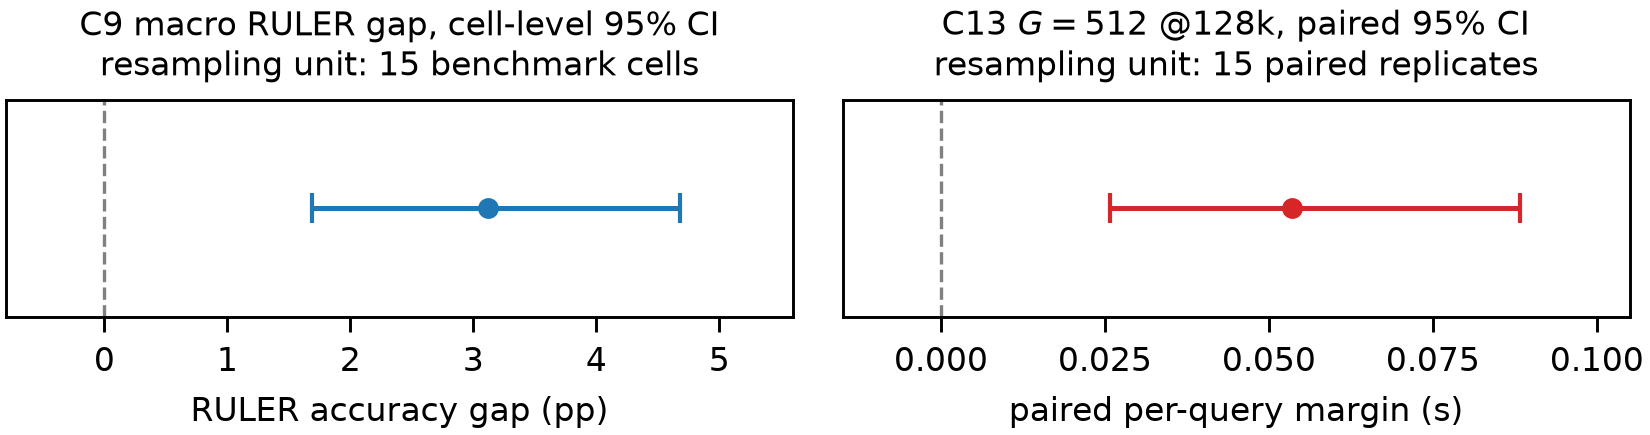
\includegraphics[width=\linewidth]{figures/fig_ci_forest.png}
  \caption{The two interval estimates this note cites, each with its own resampling population.
  \textbf{Left:} the C9 macro RULER gap, cell-level $95\%$ percentile bootstrap $[1.69,4.68]$\,pp
  (15 cells, seed 123, $n_{\mathrm{boot}}{=}20000$). \textbf{Right:} the \emph{dispersion} of the
  C13 $G{=}512$ @128k per-query margin, paired bootstrap $[0.026,0.088]$\,s (15 units). The right
  panel is a dispersion measure; the citable point margin is the recomputable aggregate figure
  $0.0404$\,s/q (Table~\ref{tab:frozen} C13). Neither interval includes zero; the axes differ
  because the quantities differ.}
  \label{fig:ci}
\end{figure}

\section{Full Notation and Ledger-ID Glossary}\label{app:notation}
The row definitions that were removed from the main-text notation table (Table~\ref{tab:notation})
to meet the page budget are collected here for completeness; they are the same definitions the
archive used.

\begin{table}[!ht]
\centering
\caption{Full notation and internal identifiers. Identifier families (C, D, S, R) index the
archived claim ledger. Rows are grouped as terms, then identifier families.}
\label{tab:notation-full}
\footnotesize
\setlength{\tabcolsep}{3pt}
\begin{tabular}{@{}>{\raggedright\arraybackslash}p{2.0cm}>{\raggedright\arraybackslash}p{11.4cm}@{}}
\toprule
\textbf{Term} & \textbf{Definition} \\
\midrule
CoMem & The archived cached-memory serving system: writes one long document's layer-$j$ hidden
states once, then replays layers $j\ldots36$ per query instead of re-prefilling. \\
\addlinespace
QCMem & The vendored selector module inside the CoMem code base; source of the
\code{create\_causal\_mask} argument mismatch of Section~\ref{sec:d1}. \\
\addlinespace
$j0$ ($j{=}0$) & The \emph{full-depth} arm: nothing cached; selected raw token-id chunks replay
through all 36 layers, so its per-query read is the most expensive. \\
\addlinespace
$j12$ & The flagship \emph{cached} arm ($j{=}12$ hidden states plus a LoRA adapter
\citep{hu2022lora}); replays 24 layers. \\
\addlinespace
B-only & The full-context (dense) baseline measured \emph{without} the LoRA adapter (arm B); the
matched adapter arm (A) was unrecoverable, so every staircase cell is B-only. \\
\addlinespace
$S$ & Per-query CPU cost of the chunk-\emph{selection} step (iterated BM25 scoring); an
algorithmic estimate, never measured on the frozen corpus. \\
\addlinespace
$G$ & Concurrency (in-flight requests), or the generated sequence length in the archived
decode model, as labelled per row. \\
\addlinespace
$Q^{*}$ & Break-even query count at which the cached arm's amortized cost falls below the
full-depth arm's; defined by Eq.~\ref{eq:qstar}. \\
\midrule
C4, C7, C9, C13 & Stable claim IDs of the archived ledger (serving cost; capacity staircase;
RULER quality; crossover), so each frozen value maps to its record. \\
\addlinespace
D1--D6 & The six decisive-evidence debts recorded at closure and their scope: D1 concurrent
full-context serving @$L{=}32$k (measured fix-and-rerun), D1-16k the same @$L{=}16$k (unmeasured
re-run), D2 adapter-source recovery, D3 KV-selector ($j0$) finite fetch, D4 adapter-identity
table completeness, D5 adapter-identity per-row binding caveat, D6 LongEval per-item re-run.
Single-arm isolation is class S1 (below), not D5. \\
\addlinespace
S1, S3, S6 & Three soundness-deficit classes from the review taxonomy: S1 the titled mechanism
was never isolated by a single arm; S3 $n{=}1$ treated as an effect; S6 no control-family member
was run. \\
\addlinespace
R142 & The internal round at which the flagship $j{=}12$ adapter arm was withdrawn; recorded in
later run configurations as \code{adapter=NONE\_WITHDRAWN\_R142}. \\
\addlinespace
``0 data'' & A GPU burn-ledger column counting \emph{usable measurement records} from one job;
``0 data across five fires'' means five GPU jobs were charged and none produced one. \\
\bottomrule
\end{tabular}
\end{table}
\end{document}
